\documentclass[12pt,oneside]{book}

\usepackage[a4paper,margin=1in]{geometry}
\usepackage{graphicx}
\usepackage{hyperref}
\usepackage{booktabs}
\usepackage{longtable}
\usepackage{array}
\usepackage{listings}
\usepackage{xcolor}
\usepackage{tikz}
\usetikzlibrary{arrows.meta,positioning,shapes.geometric}
\usepackage{float}
\usepackage{caption}
\usepackage{subcaption}
\usepackage{enumitem}
\usepackage{setspace}
\usepackage{fancyhdr}

\hypersetup{
    colorlinks=true,
    linkcolor=blue,
    citecolor=blue,
    urlcolor=blue,
    pdftitle={Medical App V3 Graduation Project Book},
    pdfauthor={Graduation Project Team}
}

\definecolor{codegray}{RGB}{245,245,245}
\definecolor{codetext}{RGB}{34,34,34}
\lstset{
    backgroundcolor=\color{codegray},
    basicstyle=\ttfamily\small\color{codetext},
    breaklines=true,
    frame=single,
    columns=fullflexible,
    keepspaces=true,
    captionpos=b
}

\setstretch{1.25}
\pagestyle{fancy}
\fancyhf{}
\fancyhead[L]{Medical App V3}
\fancyhead[R]{Graduation Project Book}
\fancyfoot[C]{\thepage}

\begin{document}

\begin{titlepage}
    \centering
    \vspace*{1.5cm}
    {\Huge\bfseries Medical App V3\par}
    \vspace{0.5cm}
    {\Large A Full-Stack Medical Monitoring and AI-Assisted Signal Analysis System\par}
    \vspace{1.5cm}
    {\large Graduation Project Book\par}
    \vfill
    {\large Department of Computer Science / Software Engineering\par}
    {\large \today\par}
\end{titlepage}

\frontmatter
\tableofcontents
\listoffigures
\listoftables

\chapter*{Internal Analysis Report}
\addcontentsline{toc}{chapter}{Internal Analysis Report}

This report summarizes the implementation facts detected before writing the graduation project book. The book content is based on the project files in the repository and avoids adding unsupported claims where the code does not provide evidence.

\begin{longtable}{p{0.27\textwidth} p{0.66\textwidth}}
\caption{Pre-writing project analysis summary}\\
\toprule
\textbf{Item} & \textbf{Detected evidence}\\
\midrule
\endfirsthead
\toprule
\textbf{Item} & \textbf{Detected evidence}\\
\midrule
\endhead
Detected project type & Full-stack medical monitoring system with Flutter frontend, FastAPI backend, PostgreSQL database, ESP32 firmware, and local AI model artifacts.\\
Detected technologies & Flutter/Dart, FastAPI, SQLAlchemy, Alembic, PostgreSQL, JWT authentication, Pydantic validation, TensorFlow/Keras model adapters, Python signal-processing services, Arduino/ESP32 firmware, MAX30105 PPG sensor, ECG analog input, pytest, and Flutter tests.\\
Main modules & Authentication, patient profile, doctor workflow, appointments, contacts, reminders, medical records, prescriptions, lab results, catalogs, admin dashboard, ECG/PPG device ingestion, session analysis, AI inference, signal chart visualization, and medical chat integration through Gemini configuration.\\
User roles & Patient, doctor, and admin. The code enforces role-specific access in patient, appointment, alert, medical-record, prescription, lab-result, device-assignment, and admin routes.\\
Main features & User registration/login, role-based navigation, profile editing, doctor selection, patient management, appointment scheduling, reminder and contact management, ECG/PPG session listing, device assignment, signal charts, AI metrics, alerts, and clinical decision-support disclaimers.\\
Database structure & SQLAlchemy models define users, emergencies, posts, votes, contacts, reminders, appointments, medical records, prescriptions, lab results, clinics, medications, devices, sessions, raw readings, analysis results, and clinical alerts. Alembic migration files exist under \texttt{Backend-bisho/DB/versions}.\\
Suggested chapter focus & The book should emphasize a medical IoT pipeline: hardware acquisition, backend validation and persistence, AI-assisted signal interpretation, role-based clinical workflows, and Flutter visualization.\\
Missing or limited information & No formal deployment descriptor, no screenshots prepared for the thesis folder, no verified clinical trial results, and no evidence of regulatory approval. These must be presented as limitations or future work, not as completed achievements.\\
\bottomrule
\end{longtable}


\mainmatter
\chapter{Abstract}

Medical App V3 is a full-stack medical monitoring graduation project designed to connect patient-facing mobile workflows with ECG and PPG signal acquisition, backend persistence, and AI-assisted physiological analysis. The system addresses a practical problem in remote and semi-continuous health monitoring: physiological readings collected from hardware devices are often difficult to organize, interpret, and present to patients or doctors in a usable software workflow. The implemented project proposes an integrated solution composed of an ESP32-based sensing layer, a FastAPI backend, a PostgreSQL relational database, local Keras model adapters, and a Flutter application for patients, doctors, and administrators.

The hardware firmware samples ECG and PPG values at 250 Hz, groups them into batches, estimates sensor state metadata such as finger detection and PPG availability, and sends JSON payloads to the backend. The backend validates incoming readings with Pydantic schemas, stores sessions and raw readings through SQLAlchemy models, optionally queues analysis jobs, and generates decision-support outputs using deterministic signal processing and optional local AI models. The Flutter frontend presents authentication, profile management, patient and doctor workflows, appointment scheduling, reminders, contacts, device assignment, session listing, ECG/PPG charts, metrics, alerts, and AI summaries.

The project demonstrates an end-to-end medical software architecture that combines mobile usability, IoT data collection, relational persistence, role-aware APIs, and AI-assisted analysis. Its expected impact is to provide a technically coherent prototype for monitoring cardiovascular signals and supporting clinical review. The implementation explicitly states that AI results are decision-support only and not a final medical diagnosis, which is an important limitation and safety boundary for academic and practical evaluation.

\chapter{Introduction}

Digital health systems increasingly rely on the integration of mobile applications, connected sensors, backend services, and data-driven decision-support methods. Cardiovascular monitoring is a particularly important application area because ECG and PPG signals can provide useful information about heart rhythm, pulse rate, signal quality, oxygen saturation estimates, and other physiological indicators. However, these signals are only useful when they are acquired reliably, validated carefully, stored consistently, and presented in a form that patients and doctors can understand.

Medical App V3 was developed as a graduation project to demonstrate such an integrated system. The project is not limited to a static patient record application. It combines a Flutter application with a FastAPI backend, a PostgreSQL database, local AI model artifacts, and ESP32 firmware for ECG/PPG acquisition. The system therefore covers several software engineering concerns at once: user authentication, role-based workflows, REST API design, database modeling, signal processing, AI model integration, and mobile visualization.

The motivation of the project is to reduce the gap between raw physiological data and practical health monitoring workflows. A patient can use the application to manage health-related information such as reminders, contacts, assigned doctors, appointments, and heart monitoring sessions. A doctor can manage patients and appointments and review related clinical information. The backend supports administrative and catalog features, while the ECG/PPG pipeline stores hardware readings and generates analysis results with explicit medical disclaimers.

\section{Overview of the Proposed System}

The proposed system follows a layered architecture. The first layer is the sensing layer, represented by ESP32 firmware that reads an ECG analog channel and MAX30105 PPG readings. The second layer is the backend service, which exposes REST endpoints, validates payloads, enforces authentication and authorization, stores data, and invokes signal analysis services. The third layer is the mobile frontend, written in Flutter, which consumes backend APIs and displays user-specific workflows and monitoring results. AI model artifacts are integrated as optional local Keras adapters, allowing the system to degrade gracefully when model dependencies are unavailable.

\section{Book Organization}

This book is organized into fourteen chapters. After this introduction, Chapter 3 defines the problem statement, Chapter 4 presents the objectives, and Chapter 5 reviews the background and related technologies. Chapters 6 and 7 analyze requirements and system workflows. Chapters 8 and 9 describe architecture and database design. Chapter 10 explains implementation details based on the actual code. Chapter 11 presents testing and evaluation, Chapter 12 discusses results, Chapter 13 concludes the project and proposes future work, and Chapter 14 provides appendices including API and installation material.

\chapter{Problem Statement}

Healthcare monitoring applications often face a disconnect between data collection and practical clinical use. Raw ECG and PPG measurements may be produced by wearable or embedded devices, but the readings must be transmitted, validated, persisted, analyzed, and displayed before they can support patient or doctor decisions. Without an integrated system, users may be left with isolated hardware readings, inconsistent records, or charts without context.

The problem addressed by Medical App V3 is the need for a unified medical monitoring platform that connects patient management, doctor workflows, and ECG/PPG signal monitoring. The project must support ordinary application functions such as login, profile management, appointments, contacts, and reminders, while also handling specialized data from hardware sensors. The software solution must therefore manage both administrative medical information and time-series physiological data.

\section{Current Challenges}

The source code indicates several practical challenges that the project attempts to solve:

\begin{itemize}[leftmargin=*]
    \item Sensor readings can be invalid because of missing finger contact, disconnected ECG leads, PPG sensor failure, or low-information signals.
    \item Large raw signal payloads can increase storage costs and response sizes unless capped or compacted.
    \item AI model dependencies may be unavailable in lightweight development or deployment environments.
    \item Different users require different access rules: patients should see their own information, doctors should manage assigned patients, and admins require broader visibility.
    \item Medical AI outputs must be presented as decision support rather than final diagnosis.
\end{itemize}

\section{Need for a Software Solution}

A software solution is needed because hardware alone cannot provide authentication, long-term storage, clinical context, or doctor-patient workflows. Similarly, a mobile application alone cannot produce reliable signal analysis without a backend capable of receiving readings, validating input, storing data, and running signal-processing services. Medical App V3 fills this gap by connecting the sensing device, backend, database, AI services, and Flutter application into a coherent prototype.

\section{Project Gap}

The gap filled by the project is an academic prototype for medical IoT monitoring that is broader than a simple CRUD application and more user-oriented than a signal-processing script. It demonstrates how physiological data can move from an ESP32 device into persistent storage, through a signal-analysis pipeline, and finally into mobile views designed for patients, doctors, and administrators.

\chapter{Project Objectives}

\section{General Objective}

The general objective of Medical App V3 is to design and implement a full-stack medical monitoring system that supports patient and doctor workflows while receiving, storing, analyzing, and visualizing ECG/PPG readings from a connected hardware device.

\section{Specific Objectives}

\begin{enumerate}[leftmargin=*]
    \item Build a Flutter application with authentication, role-aware navigation, profile screens, patient screens, doctor screens, appointments, contacts, reminders, and ECG/PPG monitoring views.
    \item Implement a FastAPI backend that exposes REST APIs for user management, clinical workflows, catalogs, administration, device ingestion, session analysis, and alerts.
    \item Design a PostgreSQL database schema using SQLAlchemy models and Alembic migrations.
    \item Implement ESP32 firmware that reads ECG and PPG signals, detects sensor states, estimates SpO2 metadata, and uploads readings to the backend.
    \item Integrate deterministic signal-processing algorithms for peak detection, heart rate, PPG rate, HRV, perfusion index, signal quality, and alert generation.
    \item Integrate optional AI adapters for ECG record classification, beat-level morphology classification, and PPG-based blood-pressure estimation.
    \item Provide tests for backend endpoints, signal processing, AI integration behavior, and Flutter model parsing.
\end{enumerate}

\section{Functional Goals}

The functional goals include registration, login, JWT token storage, profile editing, doctor selection, patient management, appointment scheduling, reminders, contacts, medical records, prescriptions, lab results, device registration, device assignment, session browsing, readings retrieval, analysis execution, and alert handling.

\section{Technical Goals}

The technical goals include modular backend routing, validated request models, relational persistence, role-based authorization, configurable environment variables, hardware token support for device ingestion, graceful AI fallback, and mobile API abstraction through a centralized Flutter service class.

\section{Academic Goals}

The academic goals are to demonstrate the ability to analyze a real problem domain, design a multi-layer architecture, implement a working prototype, evaluate it through tests and manual scenarios, and document its limitations responsibly.

\chapter{Literature Review and Background}

Medical App V3 combines ideas from mobile health, IoT sensing, backend API systems, relational databases, and machine learning based signal analysis. This chapter reviews the technologies and background concepts that support the implemented design.

\section{Mobile Health and Remote Monitoring}

Mobile health applications are commonly used to extend healthcare interaction beyond hospital visits. In this project, Flutter is used to build a cross-platform mobile interface \cite{flutter}. Flutter is suitable for the project because it supports a single Dart codebase for multiple platforms and provides rich UI components for charts, lists, forms, and role-specific screens. The implementation uses Flutter views for login, signup, home, settings, scheduled reminders, contacts, profile, doctor screens, patient screens, and ECG/PPG session visualization.

\section{Backend APIs for Medical Applications}

FastAPI is used as the backend framework \cite{fastapi}. It supports Python type annotations, Pydantic request validation, dependency injection, and automatic API documentation. These features fit the project because the backend must validate structured medical and signal payloads. For example, the \texttt{ReadingCreate} schema validates sampling rate limits, battery range, finite signal values, and matching ECG/PPG array lengths.

\section{Relational Persistence}

The backend uses SQLAlchemy models and PostgreSQL-oriented configuration for persistence \cite{sqlalchemy,postgresql}. A relational database is appropriate because the application contains structured relationships among users, doctors, patients, appointments, medical records, prescriptions, devices, sessions, readings, analysis results, and alerts. The code also includes Alembic migrations, which support controlled schema evolution.

\section{ECG and PPG Signal Analysis}

ECG and PPG signals are common physiological measurements. ECG can represent electrical cardiac activity, while PPG can reflect optical pulse changes. Public resources such as PhysioNet and the MIT-BIH Arrhythmia Database have influenced research in ECG analysis and arrhythmia classification \cite{physionet,mitbih}. Medical App V3 does not claim clinical validation against these datasets inside the repository; instead, it includes local Keras artifacts and adapters that perform decision-support classification when available.

\section{Machine Learning Integration}

TensorFlow/Keras is used for the local model artifacts \cite{tensorflow}. The backend defines three model adapters: \texttt{ecg\_arrhythmia\_v31}, \texttt{morphology\_heartbeat\_v1}, and \texttt{bp\_vital\_meta}. The implementation is designed to handle unavailable models by returning structured degraded results rather than failing the entire API response. This design is important in academic prototypes because model dependencies may not always be installed during testing.

\section{Security Background}

The backend uses JWT access tokens for authentication, following a common token-based API model \cite{jwt}. The code uses FastAPI's OAuth2 password bearer dependency pattern, which is related to OAuth2 bearer-token conventions \cite{oauth2}. Password hashing is implemented with bcrypt through Passlib. The device ingestion API can additionally require an \texttt{X-Device-Token} header when configured.

\section{Comparison with the Proposed System}

Existing systems may focus on only one layer, such as a wearable device, a mobile UI, or an AI classifier. Medical App V3 is distinctive as a graduation project because it connects all layers in one codebase. Its limitation is that it is still a prototype: the repository does not include clinical validation, production deployment scripts, regulatory documentation, or complete user-study results.

\chapter{Requirements Analysis}

Requirements were extracted from the Flutter screens, backend routers, schemas, models, tests, firmware, and README file.

\section{User Roles}

\begin{table}[H]
\centering
\caption{Detected user roles}
\begin{tabular}{p{0.2\textwidth} p{0.65\textwidth}}
\toprule
\textbf{Role} & \textbf{Responsibilities and access}\\
\midrule
Patient & Register, login, update profile, select doctor, manage reminders and contacts, view assigned device/session information, and view personal monitoring results.\\
Doctor & Manage assigned patients, create and manage appointments, view related medical information, assign devices to permitted patients, and resolve eligible alerts.\\
Admin & Access dashboard statistics, list users, manage wider device assignment, and view broader system information.\\
\bottomrule
\end{tabular}
\end{table}

\section{Functional Requirements}

\begin{longtable}{p{0.16\textwidth} p{0.74\textwidth}}
\caption{Functional requirements}\\
\toprule
\textbf{ID} & \textbf{Requirement}\\
\midrule
\endfirsthead
\toprule
\textbf{ID} & \textbf{Requirement}\\
\midrule
\endhead
FR1 & The system shall allow users to register with profile information, role, contact information, doctor data, and emergency contact data.\\
FR2 & The system shall authenticate users through a login endpoint and store bearer tokens in the Flutter client using shared preferences.\\
FR3 & The system shall route users to doctor or patient home screens based on the authenticated profile role.\\
FR4 & The system shall allow users to view and update their own profile.\\
FR5 & The system shall allow doctors to create, view, update, and delete patients assigned to them.\\
FR6 & The system shall allow doctors to create and manage appointments.\\
FR7 & The system shall allow patients to manage contacts and reminders.\\
FR8 & The system shall allow medical records, prescriptions, and lab results to be created and retrieved under role-aware authorization rules.\\
FR9 & The system shall receive ECG/PPG readings from a device through \texttt{/api/readings}.\\
FR10 & The system shall validate signal arrays, sampling rates, battery values, and matching ECG/PPG lengths before storage.\\
FR11 & The system shall store devices, monitoring sessions, raw readings, analysis results, and clinical alerts.\\
FR12 & The system shall analyze sessions and return metrics, signal quality, model predictions, alerts, and disclaimers.\\
FR13 & The Flutter application shall list monitoring sessions, display ECG/PPG charts, show metrics, and allow manual analysis execution.\\
FR14 & The backend shall return device commands such as sensor-contact checks, low-battery warning, retry capture, clinical review, or continue sampling.\\
\bottomrule
\end{longtable}

\section{Non-Functional Requirements}

\begin{table}[H]
\centering
\caption{Non-functional requirements}
\begin{tabular}{p{0.22\textwidth} p{0.63\textwidth}}
\toprule
\textbf{Quality} & \textbf{Requirement}\\
\midrule
Security & Passwords shall be hashed, authenticated routes shall require bearer tokens, and optional device ingestion tokens shall protect hardware upload endpoints.\\
Usability & The Flutter app shall provide loading, error, retry, empty, and role-specific states.\\
Reliability & Duplicate readings shall be controlled through a unique session-timestamp constraint. Invalid or low-information signals shall be compacted or flagged.\\
Maintainability & Backend functionality shall be organized into routers, schemas, models, and service modules.\\
Scalability & The database shall use indexes for common lookup fields such as device, session, timestamp, and analysis creation time.\\
Safety & AI output shall include a decision-support disclaimer and shall not be presented as final diagnosis.\\
\bottomrule
\end{tabular}
\end{table}

\section{System Constraints}

The backend depends on configured database credentials and optional model directories. The blood-pressure model requires patient metadata such as positive height and weight. Hardware upload depends on Wi-Fi configuration and sensor wiring. Formal clinical validation and regulatory approval are outside the current repository evidence and must be considered future work.

\chapter{System Analysis}

\section{Main Actors}

The main actors are patient, doctor, admin, ESP32 hardware device, and backend analysis services. The patient uses the application for personal health-management tasks and monitoring views. The doctor manages assigned patients and appointments. The admin accesses broader management information. The hardware device uploads readings. The analysis services process stored sessions and produce metrics and alerts.

\section{Use Case Overview}

\begin{longtable}{p{0.22\textwidth} p{0.25\textwidth} p{0.43\textwidth}}
\caption{Main use cases}\\
\toprule
\textbf{Use case} & \textbf{Actor} & \textbf{Description}\\
\midrule
\endfirsthead
\toprule
\textbf{Use case} & \textbf{Actor} & \textbf{Description}\\
\midrule
\endhead
Authenticate & Patient, doctor, admin & User logs in and receives a JWT access token.\\
Manage profile & Patient, doctor & User retrieves and updates personal information.\\
Manage patients & Doctor & Doctor creates, views, edits, or deletes patient entries where permitted.\\
Manage appointments & Doctor & Doctor creates and updates appointments for patients.\\
Manage reminders & Patient & Patient creates, updates, lists, and deletes reminders.\\
Upload readings & Hardware device & ESP32 sends ECG/PPG arrays and metadata to the backend.\\
Analyze session & User or worker & Backend analyzes session readings and stores an analysis result.\\
View heart session & Patient, doctor, admin & Flutter app retrieves sessions, readings, and analysis for chart display.\\
Resolve alert & Doctor, admin & Authorized user marks a clinical alert as resolved.\\
\bottomrule
\end{longtable}

\section{Data Flow}

Figure \ref{fig:data-flow} summarizes the main data path.

\begin{figure}[H]
\centering
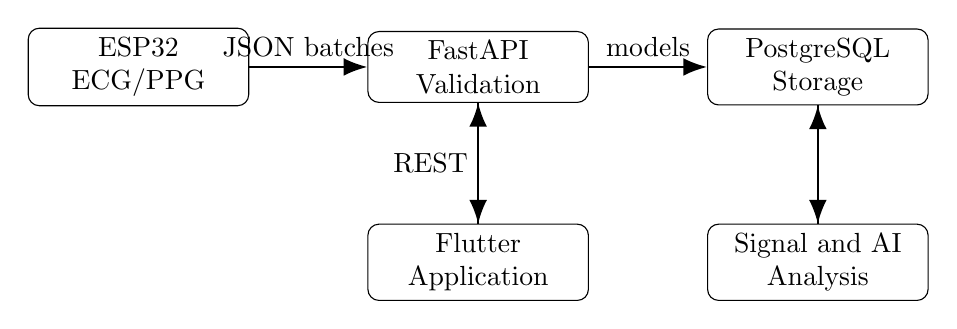
\begin{tikzpicture}[
    node distance=1.5cm,
    box/.style={rectangle,draw,rounded corners,align=center,minimum width=2.8cm,minimum height=0.9cm},
    arrow/.style={-{Latex[length=3mm]},thick}
]
\node[box] (sensor) {ESP32\\ECG/PPG};
\node[box,right=of sensor] (api) {FastAPI\\Validation};
\node[box,right=of api] (db) {PostgreSQL\\Storage};
\node[box,below=of db] (ai) {Signal and AI\\Analysis};
\node[box,left=of ai] (app) {Flutter\\Application};
\draw[arrow] (sensor) -- node[above]{JSON batches} (api);
\draw[arrow] (api) -- node[above]{models} (db);
\draw[arrow] (db) -- (ai);
\draw[arrow] (ai) -- (db);
\draw[arrow] (app) -- node[left]{REST} (api);
\draw[arrow] (api) -- (app);
\end{tikzpicture}
\caption{End-to-end data flow from hardware to mobile visualization}
\label{fig:data-flow}
\end{figure}

\section{Workflow Description}

The ECG/PPG monitoring workflow begins when the ESP32 firmware samples ECG and PPG data. It forms a batch, evaluates sensor status, builds a JSON payload, and posts it to \texttt{/api/readings}. The backend validates the request, creates the device and session if needed, prepares storage by compacting invalid signals when configured, stores the raw reading, and returns device commands. A user can later request analysis with \texttt{/api/analyze/\{session\_id\}}, or automatic analysis can be queued if enabled. The Flutter app retrieves sessions, readings, and analysis results and displays signal charts, metrics, signal quality, alerts, and disclaimers.

\chapter{System Design and Architecture}

\section{Overall Architecture}

Medical App V3 uses a layered architecture. The frontend is implemented in Flutter under the \texttt{lib} directory. The backend is implemented in FastAPI under \texttt{Backend-bisho}. The database layer is represented by SQLAlchemy models and Alembic migrations. The hardware layer is represented by firmware under \texttt{hardware/ECG\_PPG\_HR\_SPO2}. AI artifacts are stored under \texttt{AI models}.

\begin{figure}[H]
\centering
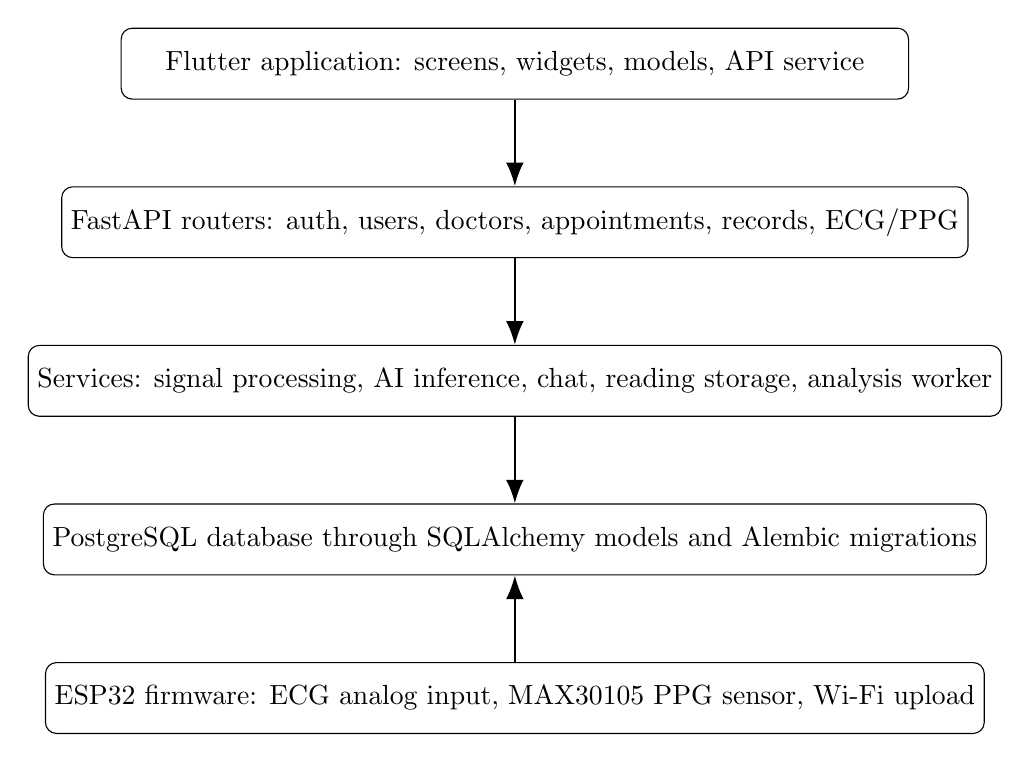
\begin{tikzpicture}[
    node distance=1.1cm,
    layer/.style={rectangle,draw,rounded corners,align=center,minimum width=10cm,minimum height=0.9cm},
    arrow/.style={-{Latex[length=3mm]},thick}
]
\node[layer] (ui) {Flutter application: screens, widgets, models, API service};
\node[layer,below=of ui] (api) {FastAPI routers: auth, users, doctors, appointments, records, ECG/PPG};
\node[layer,below=of api] (service) {Services: signal processing, AI inference, chat, reading storage, analysis worker};
\node[layer,below=of service] (data) {PostgreSQL database through SQLAlchemy models and Alembic migrations};
\node[layer,below=of data] (hardware) {ESP32 firmware: ECG analog input, MAX30105 PPG sensor, Wi-Fi upload};
\draw[arrow] (ui) -- (api);
\draw[arrow] (api) -- (service);
\draw[arrow] (service) -- (data);
\draw[arrow] (hardware) -- (data);
\end{tikzpicture}
\caption{Layered architecture of Medical App V3}
\label{fig:architecture}
\end{figure}

\section{Frontend Structure}

The Flutter code separates authentication pages, home pages, doctor screens, patient screens, shared widgets, models, configuration, and API communication. The \texttt{ApiService} class centralizes HTTP calls and token storage. The application entry point loads settings, applies theme/font direction preferences, and uses an authentication gate to choose between login, patient home, or doctor home.

\section{Backend Structure}

The backend includes:

\begin{itemize}[leftmargin=*]
    \item \texttt{app/main.py}: FastAPI application creation, CORS middleware, router registration, and lifecycle startup/shutdown for the analysis worker.
    \item \texttt{app/models.py}: SQLAlchemy entities.
    \item \texttt{app/schemas.py}: Pydantic request and response models.
    \item \texttt{routers}: REST endpoints grouped by domain.
    \item \texttt{app/services}: signal processing, AI inference, reading storage, background analysis, chat service, and prompt definitions.
\end{itemize}

\section{Authentication and Authorization}

Authentication uses login credentials and JWT access tokens. The backend creates tokens with a user identifier and expiration. Protected routes depend on \texttt{get\_current\_user}. Authorization is role-aware: doctors can access assigned patients, patients are restricted to their own information, and admin users receive broader privileges. Device ingestion has a separate optional token using the \texttt{X-Device-Token} header.

\section{Error Handling and Degraded AI}

The backend handles invalid schemas with Pydantic validation errors, missing records with HTTP 404 responses, unauthorized access with HTTP 401 or 403 responses, and invalid capture state with HTTP 400 responses. AI model calls are wrapped in timeout and retry logic. If TensorFlow artifacts or metadata are unavailable, the analysis response is marked as degraded rather than failing the whole session analysis.

\section{Deployment Overview}

The README describes development deployment using PostgreSQL, Alembic migrations, FastAPI on port 8000, Flutter with \texttt{BACKEND\_BASE\_URL}, and Arduino firmware configured through \texttt{config.h}. No production container, cloud deployment, or continuous deployment configuration was found, so production deployment is treated as future work.

\chapter{Database Design}

The database design is implemented through SQLAlchemy models in \texttt{Backend-bisho/app/models.py}. The schema supports user management, doctor-patient relationships, clinical workflow data, hardware devices, monitoring sessions, raw readings, analysis results, and alerts.

\section{Main Entities}

\begin{longtable}{p{0.22\textwidth} p{0.24\textwidth} p{0.44\textwidth}}
\caption{Important database tables}\\
\toprule
\textbf{Table} & \textbf{Key fields} & \textbf{Purpose}\\
\midrule
\endfirsthead
\toprule
\textbf{Table} & \textbf{Key fields} & \textbf{Purpose}\\
\midrule
\endhead
\texttt{users} & \texttt{id}, \texttt{email}, \texttt{role}, \texttt{doc\_id}, \texttt{emergency\_id} & Stores patient, doctor, and admin accounts.\\
\texttt{emergencys} & \texttt{id}, \texttt{name}, \texttt{email}, \texttt{phone\_number} & Stores emergency contact data.\\
\texttt{contacts} & \texttt{id}, \texttt{owner\_id} & Stores patient contact entries.\\
\texttt{reminders} & \texttt{id}, \texttt{owner\_id}, \texttt{date}, \texttt{time\_hour} & Stores reminders.\\
\texttt{appointments} & \texttt{id}, \texttt{doctor\_id}, \texttt{patient\_id} & Stores appointment records.\\
\texttt{medical\_records} & \texttt{id}, \texttt{patient\_id}, \texttt{doctor\_id} & Stores diagnosis and notes with metadata JSON.\\
\texttt{prescriptions} & \texttt{id}, \texttt{appointment\_id}, \texttt{patient\_id}, \texttt{doctor\_id} & Stores medication prescriptions.\\
\texttt{lab\_results} & \texttt{id}, \texttt{appointment\_id}, \texttt{patient\_id}, \texttt{doctor\_id} & Stores laboratory result entries.\\
\texttt{clinics} & \texttt{id}, \texttt{name}, \texttt{specialty} & Stores clinic catalog data.\\
\texttt{medications} & \texttt{id}, \texttt{name}, \texttt{category} & Stores medication catalog data.\\
\texttt{devices} & \texttt{id}, \texttt{device\_id}, \texttt{patient\_id} & Stores hardware device identities and assignment.\\
\texttt{sessions} & \texttt{id}, \texttt{session\_id}, \texttt{device\_id}, \texttt{patient\_id} & Stores monitoring sessions.\\
\texttt{raw\_readings} & \texttt{id}, \texttt{device\_id}, \texttt{session\_id}, \texttt{timestamp} & Stores ECG/PPG arrays and sensor metadata.\\
\texttt{analysis\_results} & \texttt{id}, \texttt{session\_id}, \texttt{metrics}, \texttt{predictions} & Stores signal and AI analysis outputs.\\
\texttt{clinical\_alerts} & \texttt{id}, \texttt{patient\_id}, \texttt{session\_id}, \texttt{analysis\_id} & Stores analysis-generated alerts and resolution status.\\
\bottomrule
\end{longtable}

\section{Relationships}

Users can reference another user as a doctor through \texttt{doc\_id}. Devices can be assigned to patients. Monitoring sessions belong to devices and optionally to patients. Raw readings belong to sessions and devices. Analysis results belong to sessions. Clinical alerts can reference patients, sessions, and analysis results. Appointments, prescriptions, medical records, and lab results connect doctors and patients.

\begin{figure}[H]
\centering
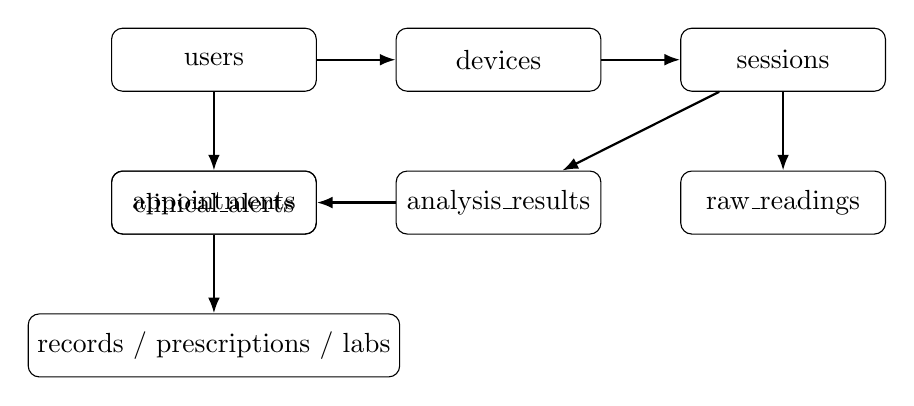
\begin{tikzpicture}[
    entity/.style={rectangle,draw,rounded corners,align=center,minimum width=2.6cm,minimum height=0.8cm},
    arrow/.style={-{Latex[length=2mm]},thick}
]
\node[entity] (user) {users};
\node[entity,right=of user] (device) {devices};
\node[entity,right=of device] (session) {sessions};
\node[entity,below=of session] (reading) {raw\_readings};
\node[entity,left=of reading] (analysis) {analysis\_results};
\node[entity,left=of analysis] (alerts) {clinical\_alerts};
\node[entity,below=of user] (appt) {appointments};
\node[entity,below=of appt] (clinical) {records / prescriptions / labs};
\draw[arrow] (user) -- (device);
\draw[arrow] (device) -- (session);
\draw[arrow] (session) -- (reading);
\draw[arrow] (session) -- (analysis);
\draw[arrow] (analysis) -- (alerts);
\draw[arrow] (user) -- (appt);
\draw[arrow] (appt) -- (clinical);
\end{tikzpicture}
\caption{Simplified ERD for main clinical and monitoring tables}
\label{fig:erd}
\end{figure}

\section{Constraints and Indexes}

The \texttt{raw\_readings} table has a unique constraint on \texttt{session\_id} and \texttt{timestamp}, preventing duplicate packet corruption. Indexes are defined for session, device, timestamp, and analysis timestamps. Pydantic schemas complement database constraints by validating signal arrays, finite numbers, battery range, and sampling rate before data reaches the database.

\chapter{Implementation}

\section{Technology Stack}

The implementation uses Flutter and Dart for the frontend, FastAPI and Python for the backend, SQLAlchemy and Alembic for database access and migration, PostgreSQL for persistence, TensorFlow/Keras for optional AI model inference, and Arduino/ESP32 firmware for sensor acquisition. The Flutter application depends on packages such as \texttt{http}, \texttt{shared\_preferences}, \texttt{flutter\_local\_notifications}, \texttt{timezone}, \texttt{url\_launcher}, \texttt{image\_picker}, \texttt{google\_maps\_flutter}, and \texttt{geolocator}.

\section{Project Folder Structure}

\begin{lstlisting}[caption={Main repository structure}]
lib/                         Flutter source code
Backend-bisho/app/           FastAPI app, models, schemas, services
Backend-bisho/routers/       API routers
Backend-bisho/DB/versions/   Alembic migrations
AI models/                   Local Keras/scaler artifacts
hardware/ECG_PPG_HR_SPO2/    ESP32 firmware
docs/                        Sample payload and Postman collection
test/                        Flutter model tests
Backend-bisho/tests/         Backend pytest tests
\end{lstlisting}

\section{Frontend Implementation}

The Flutter entry point initializes settings, loads the theme and text direction, and runs an \texttt{AuthGate}. The authentication gate checks for a stored token and requests the current user profile. If the role is \texttt{doctor}, the app opens \texttt{DoctorHomeScreen}; otherwise it opens the patient home view. If token validation fails, the token is cleared and the login screen is shown.

The \texttt{ApiService} class implements token helpers, authentication, profile requests, reminders, contacts, appointments, patients, doctors, medical records, prescriptions, lab results, clinics, medications, admin statistics, and ECG/PPG pipeline calls. This central service reduces repeated HTTP logic across UI screens.

\section{ECG/PPG UI}

The \texttt{MyHeartPage} loads sessions, devices, and profile information. Doctors and admins can assign devices to patients; patients can self-assign eligible devices. A session details page retrieves session metadata, raw readings, and analysis results. It draws ECG and PPG charts using a custom painter, presents metrics, handles sensor-state warnings, and allows manual analysis execution.

\section{Backend Implementation}

The FastAPI backend registers routers for posts, users, authentication, votes, reminders, contacts, chat, patients, doctors, appointments, ECG/PPG pipeline, medical records, prescriptions, lab results, catalogs, and admin functions. CORS configuration is loaded from settings, and an analysis worker is started during application lifespan.

\section{Signal Processing Implementation}

The signal-processing service implements normalization, moving average, detrending, peak detection, rate calculation, HRV calculation, signal-quality scoring, perfusion index calculation, and alert generation. A simplified code excerpt is shown below.

\begin{lstlisting}[language=Python,caption={Peak-based metric workflow}]
ecg_filtered = detrend(ecg, sampling_rate)
ppg_filtered = detrend(ppg, sampling_rate)
ecg_peaks = detect_peaks(ecg_filtered, sampling_rate)
ppg_peaks = detect_peaks(ppg_filtered, sampling_rate)
heart_rate = calculate_rate_from_peaks(ecg_peaks, sampling_rate)
ppg_rate = calculate_rate_from_peaks(ppg_peaks, sampling_rate)
hrv = calculate_hrv(ecg_peaks, sampling_rate)
\end{lstlisting}

\section{AI Inference Implementation}

The inference service defines adapters for three models. The record-level ECG model expects at least 1250 ECG samples and produces class probability maps. The morphology model extracts beat-centered ECG windows of 186 samples. The blood-pressure model builds a PPG beat sequence at 125 Hz and uses patient metadata including weight, height, and BMI. Each adapter returns structured availability information, enabling degraded analysis when artifacts or metadata are missing.

\section{Hardware Implementation}

The ESP32 firmware samples at 250 Hz and batches 125 samples. It reads ECG through an analog pin, detects ECG leads-off state, reads IR and red values from the MAX30105 sensor, estimates finger contact, calculates a rough SpO2 value when possible, and uploads JSON to the backend. It also interprets backend command hints and prints messages for sensor contact, low battery, retry capture, clinical review, or continue sampling.

\section{Security Implementation}

Passwords are hashed with bcrypt. Users authenticate through a login route and receive JWT access tokens. Protected backend routes depend on the current user. Device uploads can be protected by \texttt{X-Device-Token}. Role checks are used in doctor, patient, admin, alert, medical-record, prescription, lab-result, and device-assignment routes.

\chapter{Testing and Evaluation}

\section{Testing Strategy}

The repository contains backend tests under \texttt{Backend-bisho/tests} and Flutter tests under \texttt{test}. The backend tests use FastAPI's \texttt{TestClient}, SQLite in-memory databases, dependency overrides, and seeded test data. The Flutter test validates parsing of backend JSON models.

\section{Implemented Automated Tests}

\begin{longtable}{p{0.22\textwidth} p{0.5\textwidth} p{0.18\textwidth}}
\caption{Detected automated tests}\\
\toprule
\textbf{Test area} & \textbf{Examples} & \textbf{Expected result}\\
\midrule
\endfirsthead
\toprule
\textbf{Test area} & \textbf{Examples} & \textbf{Expected result}\\
\midrule
\endhead
Signal processing & Peak detection, metrics, signal quality, flat normalization & Correct peaks, metrics, and stable zero output for flat signals.\\
ECG/PPG API & Session creation, reading upload, analysis, invalid payload rejection & Valid readings are stored and analyzed; invalid readings are rejected.\\
Sensor states & No finger, PPG off, leads off, large payload cap & Commands and storage compaction behave as expected.\\
AI integration & Model registry, normalized outputs, degraded short ECG, BP metadata requirements & Models are listed and degraded states are structured.\\
User endpoints & Profile patch and doctor assignment & User profile updates persist correctly.\\
Flutter models & Session and raw reading parsing & JSON fields map to Dart model properties.\\
\bottomrule
\end{longtable}

\section{Manual Test Cases}

\begin{longtable}{p{0.12\textwidth} p{0.32\textwidth} p{0.42\textwidth}}
\caption{Suggested manual test cases}\\
\toprule
\textbf{ID} & \textbf{Scenario} & \textbf{Expected result}\\
\midrule
\endfirsthead
\toprule
\textbf{ID} & \textbf{Scenario} & \textbf{Expected result}\\
\midrule
\endhead
MT1 & Register a patient account and login & Patient is routed to the patient home screen.\\
MT2 & Register or login as doctor & Doctor is routed to the doctor home screen.\\
MT3 & Create an appointment for a patient & Appointment appears in the appointment list.\\
MT4 & Upload sample reading payload & Backend creates device/session/reading and returns commands.\\
MT5 & Open My Heart page & Sessions and devices load with refresh and error states.\\
MT6 & Run analysis on valid session & Metrics, signal quality, predictions, alerts, and disclaimer appear.\\
MT7 & Upload no-finger payload & Backend drops invalid PPG and prevents analysis until contact is valid.\\
MT8 & Assign device as doctor & Device patient assignment changes only when authorization rules allow it.\\
\bottomrule
\end{longtable}

\section{Evaluation}

The tests demonstrate that the core monitoring pipeline can accept readings, reject invalid payloads, process signal metrics, preserve storage metadata, and handle model availability. The tests also evaluate safety-relevant conditions such as missing finger contact, PPG sensor failure, ECG leads-off state, and large payload capping. No formal usability study, performance benchmark, or clinical validation dataset result was found in the repository, so these remain limitations.

\chapter{Results and Discussion}

\section{Achieved Results}

Medical App V3 successfully implements a working full-stack prototype. The frontend provides role-aware application flow, medical workflow screens, and ECG/PPG visualization. The backend exposes a broad set of REST endpoints and maintains a structured relational model. The hardware firmware can produce the expected JSON format for the backend. The analysis services can compute deterministic metrics and integrate local AI models when dependencies and artifacts are available.

\section{System Behavior}

The ECG/PPG session screen displays session cards, device assignment controls, signal charts, analysis sections, quality indicators, alerts, and disclaimers. The UI accounts for empty sessions, loading states, retry states, and sensor problems. The backend returns device commands that allow the firmware to report actionable messages when the sensor state is poor.

\section{Strengths}

The main strength of the system is integration. It connects embedded sampling, REST ingestion, database persistence, AI-assisted processing, and Flutter visualization. Another strength is defensive behavior: invalid readings are not blindly trusted, AI failures are represented as degraded outputs, and analysis output includes a decision-support disclaimer. The system also demonstrates role-aware medical workflow design rather than treating all users identically.

\section{Limitations}

The repository does not include evidence of formal clinical validation, regulatory compliance, production deployment, or a usability study. Some AI outputs depend on local model artifacts and optional dependencies. The blood-pressure model requires patient height and weight metadata. Screenshots are not packaged in the thesis folder, so placeholders are used in the appendix. These limitations do not invalidate the prototype, but they define its proper academic interpretation.

\section{Discussion}

The original problem was the difficulty of connecting raw physiological readings with practical application workflows. The implemented system addresses this by creating a complete path from sensor data to mobile interpretation. The project also recognizes the risks of medical AI by avoiding diagnostic overclaiming. Therefore, the system should be viewed as an educational and technical prototype that can support review and monitoring, not as an independently certified medical device.

\chapter{Conclusion and Future Work}

\section{Conclusion}

This graduation project designed and implemented Medical App V3, a full-stack medical monitoring system that combines Flutter, FastAPI, PostgreSQL, ESP32 firmware, signal processing, and optional AI model adapters. The project supports patient, doctor, and admin workflows while also handling ECG/PPG data ingestion and analysis. The implemented architecture demonstrates practical knowledge of mobile application development, backend API design, database modeling, authentication, authorization, embedded device communication, and AI-assisted health monitoring.

The project achieved its main technical goals by connecting hardware readings to persistent sessions, exposing APIs for analysis and retrieval, displaying signal charts and metrics in Flutter, and including tests for key backend and frontend behaviors. The explicit disclaimer that AI results are decision-support only is an important part of the system's responsible design.

\section{Lessons Learned}

The project shows that medical monitoring systems require careful validation at every layer. Hardware status must be captured, invalid signal states must be handled, API schemas must reject unsafe payloads, databases must prevent duplicate readings, and user roles must be enforced consistently. It also shows that AI integration should include timeout handling, fallback behavior, and transparent status reporting.

\section{Future Work}

Future work can improve the system in the following ways:

\begin{itemize}[leftmargin=*]
    \item Add a production deployment configuration using containers, HTTPS, environment-specific settings, and database backup plans.
    \item Add formal clinical validation with approved datasets and expert review.
    \item Add more complete UI screenshots and a polished user manual.
    \item Add real-time streaming or WebSocket updates for live monitoring.
    \item Add notification workflows for alerts and appointment reminders.
    \item Expand automated tests for all clinical workflow routers and Flutter screens.
    \item Add audit logging for medical-record changes and alert resolution.
    \item Improve model governance by documenting training data, evaluation metrics, versioning, and limitations.
\end{itemize}

\chapter{Appendices}

\section{API Documentation Summary}

\begin{longtable}{p{0.28\textwidth} p{0.18\textwidth} p{0.44\textwidth}}
\caption{Selected API endpoints}\\
\toprule
\textbf{Endpoint} & \textbf{Method} & \textbf{Purpose}\\
\midrule
\endfirsthead
\toprule
\textbf{Endpoint} & \textbf{Method} & \textbf{Purpose}\\
\midrule
\endhead
\texttt{/login/} & POST & Authenticate user and return token.\\
\texttt{/users/} & POST & Register user.\\
\texttt{/users/me} & GET/PUT/PATCH & Retrieve or update current profile.\\
\texttt{/patients/} & GET & List patients for authorized doctor.\\
\texttt{/appointments/} & GET & List appointments.\\
\texttt{/appointments/createappointment/} & POST & Create appointment.\\
\texttt{/contacts/} & GET & List contacts.\\
\texttt{/reminders/} & GET & List reminders.\\
\texttt{/medical-records/patient/\{id\}} & GET & Retrieve patient medical records.\\
\texttt{/prescriptions/appointment/\{id\}} & GET & Retrieve prescriptions by appointment.\\
\texttt{/lab-results/appointment/\{id\}} & GET & Retrieve lab results by appointment.\\
\texttt{/api/sessions} & POST/GET & Create or list monitoring sessions.\\
\texttt{/api/readings} & POST & Upload ECG/PPG reading batch.\\
\texttt{/api/analyze/\{session\_id\}} & POST & Analyze a monitoring session.\\
\texttt{/api/devices} & GET & List hardware devices.\\
\texttt{/api/devices/\{device\_id\}/assign} & PATCH & Assign or unassign device.\\
\texttt{/api/alerts} & GET & List clinical alerts.\\
\texttt{/api/alerts/\{alert\_id\}/resolve} & PATCH & Resolve alert.\\
\texttt{/api/ai/models} & GET & List AI model metadata and availability.\\
\bottomrule
\end{longtable}

\section{Sample Reading Payload}

\begin{lstlisting}[caption={Sample ECG/PPG reading payload}]
{
  "device_id": "device_001",
  "session_id": "session_123",
  "timestamp": "2026-05-13T10:30:00Z",
  "sampling_rate": 250,
  "ecg": [0.12, 0.15, 0.18],
  "ppg": [520, 525, 531],
  "battery": 90,
  "status": "active"
}
\end{lstlisting}

\section{Installation Steps}

\subsection{Backend}

\begin{lstlisting}[caption={Backend setup}]
cd Backend-bisho
python -m venv .venv
.\.venv\Scripts\Activate.ps1
pip install -r requirements.txt
alembic upgrade head
uvicorn app.main:app --reload --host 0.0.0.0 --port 8000
\end{lstlisting}

\subsection{Flutter}

\begin{lstlisting}[caption={Flutter setup}]
flutter pub get
flutter run --dart-define=BACKEND_BASE_URL=http://127.0.0.1:8000
\end{lstlisting}

\subsection{Hardware}

\begin{enumerate}[leftmargin=*]
    \item Install ESP32 board support in Arduino IDE.
    \item Install the SparkFun MAX30105 library.
    \item Copy \texttt{hardware/config.example.h} to \texttt{hardware/config.h}.
    \item Configure Wi-Fi, backend URL, device ID, session ID, and pins.
    \item Upload \texttt{hardware/ECG\_PPG\_HR\_SPO2/ECG\_PPG\_HR\_SPO2.ino}.
\end{enumerate}

\section{Environment Variables}

\begin{table}[H]
\centering
\caption{Important backend and frontend configuration}
\begin{tabular}{p{0.34\textwidth} p{0.5\textwidth}}
\toprule
\textbf{Variable} & \textbf{Purpose}\\
\midrule
\texttt{DATABASE\_URL} or database fields & PostgreSQL connection configuration.\\
\texttt{SECRET\_KEY} & JWT signing secret.\\
\texttt{GEMINI\_API\_KEY} & Optional medical chat API key.\\
\texttt{DEVICE\_INGEST\_TOKEN} & Optional hardware upload token.\\
\texttt{ECG\_MODEL\_DIR} & ECG classifier model directory.\\
\texttt{MORPHOLOGY\_MODEL\_DIR} & Beat morphology model directory.\\
\texttt{BP\_MODEL\_DIR} & Blood-pressure model directory.\\
\texttt{AUTO\_ANALYZE\_ON\_UPLOAD} & Enables background analysis after upload.\\
\texttt{BACKEND\_BASE\_URL} & Flutter backend URL passed with \texttt{--dart-define}.\\
\bottomrule
\end{tabular}
\end{table}

\section{User Manual}

Patients should register, login, complete profile information, select or create a doctor, manage reminders and contacts, and open the heart monitoring page to review sessions. Doctors should login, manage patients, create appointments, review relevant records, and assign devices where authorized. Admin users can inspect dashboard statistics and wider user/device data.

\section{Screenshot Placeholders}

The repository contains image assets, but no complete thesis screenshot set was found. Add screenshots to the \texttt{figures} directory and reference them here.

\begin{figure}[H]
\centering
\fbox{\parbox{0.75\textwidth}{\centering Placeholder for login and signup screens}}
\caption{Authentication screens placeholder}
\end{figure}

\begin{figure}[H]
\centering
\fbox{\parbox{0.75\textwidth}{\centering Placeholder for ECG/PPG session and analysis screens}}
\caption{Heart monitoring screens placeholder}
\end{figure}


\backmatter
\bibliographystyle{plain}
\bibliography{references}

\end{document}
